\documentclass{article}

\usepackage[utf8]{inputenc}
\usepackage{graphicx}
\usepackage{natbib}
\usepackage{amsmath}
\usepackage{amssymb}
\usepackage{amsthm}
\usepackage{mathpartir}
\usepackage{bm}
\usepackage{hyperref}
\usepackage{cleveref}

\newcommand{\Pend}{\bm{0}}
\newcommand{\Ppar}[2]{#1 \mid #2}
\newcommand{\Pres}[2]{(\bm{\nu} #1)~#2}
\newcommand{\Pout}[3]{#1 ! #2 . #3}
\newcommand{\Pin}[3]{#1 ? (#2) . #3}
\newcommand{\Pchoice}[2]{#1 + #2}
\newcommand{\Preplicate}[1]{{!}#1}

\newcommand{\freenames}[1]{\textrm{fn}(#1)}
\newcommand{\boundnames}[1]{\textrm{bn}(#1)}
\newcommand{\names}[1]{\textrm{n}(#1)}

\newcommand{\freevars}[1]{\textrm{fv}(#1)}
\newcommand{\boundvars}[1]{\textrm{bv}(#1)}
\newcommand{\vars}[1]{\textrm{vars}(#1)}

\newcommand{\alphacon}[2]{#1 =_{\alpha} #2}
\newcommand{\subst}[3]{#1\{#2/#3\}}

\newcommand{\Aoutf}[2]{#1 ! #2}
\newcommand{\Aoutb}[2]{#1 ! (#2)}
\newcommand{\Ain}[2]{#1 ? #2}
\newcommand{\Atau}{\tau}

\newcommand{\transition}[3]{#1 \xrightarrow{#2} #3}

\newcommand{\observable}[2]{#1\downarrow_{#2}}
\newcommand{\obsin}[1]{#1?}
\newcommand{\obsout}[1]{#1!}

\newcommand\sbullet[1][.5]{\mathbin{\hbox{\scalebox{#1}{$\bullet$}}}}
\newcommand{\sbbisim}[2]{#1 \overset{\sbullet}{\sim} #2}
\newcommand{\nsbbisim}[2]{#1 \not\overset{\sbullet}{\sim} #2}

\newcommand{\ctxhole}{[\cdot]}
\newcommand{\applyctx}[2]{#1[#2]}
\newcommand{\sbcong}[2]{#1 \simeq^c #2}

\newcommand{\applysubst}[2]{#2#1}

\newcommand{\Presd}[3]{(\bm{\nu} #1#2)~#3}
\newcommand{\scong}[2]{#1 \equiv #2}

\newcommand{\reduces}[2]{#1 \rightarrow #2}

\newcommand{\Tend}{\mathbf{end}}
\newcommand{\Tbase}{\mathbf{base}}
\newcommand{\Tin}[1]{{?}.#1}
\newcommand{\Tout}[1]{{!}.#1}

\newcommand{\hastype}[2]{#1 : #2}

\newcommand{\un}[1]{\mathbf{un}(#1)}
\newcommand{\lin}[1]{\mathbf{lin}(#1)}

\newcommand{\Cempty}{\varnothing}
\newcommand{\Cadd}[2]{#1, #2}
\newcommand{\Csplit}[2]{#1 \circ #2}
\newcommand{\Cupdate}[2]{#1 + #2}

\newcommand{\dual}[1]{\overline{#1}}

\newcommand{\types}[2]{#1 \vdash #2}

%% Local Variables:
%% mode: latex
%% TeX-master: "main"
%% End:


\begin{document}

\title{POPLMark goes Concurrent!\\Challenge problems for process calculi and behavioural types}

\maketitle

\begin{abstract}
  The publication of POPLMark spearheaded the era of publishing formal
  proofs alongside with new research. This fostered an era of
  high-quality and high-assurance proofs at top venues for programming
  language research. This paper simultaneously acknowledges the impact
  of the original POPLMark challenge, and proposes a new benchmark
  intended to stimulate the research and dissemination of techniques
  that address the particular challenges of process calculi and
  behavioural type systems. In this work we propose three challenge
  problems concerning to process calculi and name passing, linearity
  in behavioural type systems, and coinductive reasoning for process
  algebras.
\end{abstract}

\section{Introduction}

In recent years, the programming language community has embraced
machine checked proofs for theoretical results in papers. The
POPLMark~\cite{Pierce:2005} challenge was proposed for this purpose,
and to get the community on track. Since then the number of formal
proofs accompanying papers has grown\footnote{add some POPL/PLDI/etc
  statistics here}. However, formal proofs are not equally spread in
the field. In this call to action, we propose to extend the key
contribution of challenges like POPLMark is to help develop the
necessary momentum and culture to be able to formalise results to the
concurrent calculi community by proposing a challenge the exercises
the key aspects of reasoning about process calculi. We propose this
document, and a \href{https://concurrentbenchmark.github.io/}{website}
to enable the community to collaborate on the project.

It has been a long time since the original challenge, and many changes
have happened. Particularly, POPLMark and any challenge cannot address
every conceivable technique. Challenges have to be simple so that the
techniques are not shadowed by technical details and also feasible to
implement without heroic efforts. In that vein, it is apparent that
new challenges are needed, work like POPLMark
Reloaded~\cite{Pientka:2019} strives to extend the scope of the
original challenge to proofs using logical relations. This technique
is crucial to many current developments.

As mentioned before, in this work we address another expansion of
scope for such challenges, going from the $\lambda$-calculus to
process calculi such as the $\pi$-calculus and session type systems
(and other behavioural type systems). These systems require particular
insights to implement. So far, we have identified three key
aspects\footnote{We want to keep the number low, but the exact nature
  of the challenges is still open to discussion (as are most things in
  this project).}. First, the idea of scope extrusion in name passing
calculi. This generalises the idea of binders in ways that techniques
that were adequate for $\lambda$-calculus binders are not so
convenient for name passing systems. Second, session types in
particular, and behavioural types in general often depend on linearity
in their type systems. The formalisation of linear type systems posses
a challenge given that it is not uniformly well supported among the
many proof assistants. Finally, processes in concurrent systems often
contain infinite behaviour that is typically modelled with
coinduction. This technique is used to reason about (bi)similarity
between processes, the equivalence of their traces, or subtyping
between infinite trees of possible behaviours. This challenge
concentrates on those issues.

In this work we propose a challenge where each part independently
exercises one of the three areas, however it is often the case that a
problem requires more than one of these techniques simultaneously. In
this work, we explore them in isolation, in order to facilitate the
implementation of smaller solutions. Concretely, we do not address the
idea of how to combine these techniques, leaving the discussion of
that to the future when we have collected enough entries to these
problems.

We do not claim in this work that these problems have never been
approached and formalised before. In fact, the contrary is true. All
of these problems have been addressed in several forms. This motivates
this challenge to enable an easier comparison between solutions (since
they all implement the same challenge), and in a setting that is
\emph{simple enough to not be distracting, yet complex enough that we can
compare strengths and weaknesses of each}.

The rest of this paper is structured in the following way:
\cref{sec:rationale} expands on the rationale for the selected
challenge problems. Then \cref{sec:problems} presents the problems. We
discuss the solutions in \cref{sec:solutions}, in particular
\cref{sec:tutorial} walks through a tutorial solution. And finally
\cref{sec:conclusion} presents some conclusions and it contains a call
to action to invite the submission of new solutions.

\section{Rationale for choosing the problems}\label{sec:rationale}

This section is not (at least initially) meant to be in the final
manuscript but it is to document some reasoning for choosing
appropriate problems. The idea is to explore three areas: scope
extrusion in name passing calculi, linearity requirements in
behavioural types, and finally coinductive reasoning in trace
equivalence, (bi)similarity, or subtyping in the presence of
recursion.

The idea is to have three small problems in the aforementioned
subjects that are independent of each other and that are easy to
understand and to implement. This is important so we have more
entries. They have to be small so it is not a lot to read, and
independent so people may choose to implement only one of them, or
work on them in any order. Moreover, the specification should only
need to be met in spirit. The idea is to provide a solution author
with some space to show the best aspects of their solution even if
that means adapting the problem definition while keeping the spirit of
the challenge.

Finally, it will be important to mention in the rationale for problems that
the key aspects are:
\begin{itemize}
\item Scope extrusion
\item Linearity
\item Coinduction
\end{itemize}

But the exact presentation of the concrete problems should be somewhat
flexible. In the sense that the use of certain techniques or tools may
require changing the presentation of the system to fit the technique.
These changes should be allowed, and even encouraged, but the result
should be ``morally'' the same system and there should be a
rationale for the changes in presentation. That way we could not only
see valid techniques but also what presentation of the rules to use
and the rationale to chose a particular approach.

\section{The challenge problems} \label{sec:problems}

\begin{figure}[h]
  \centering
  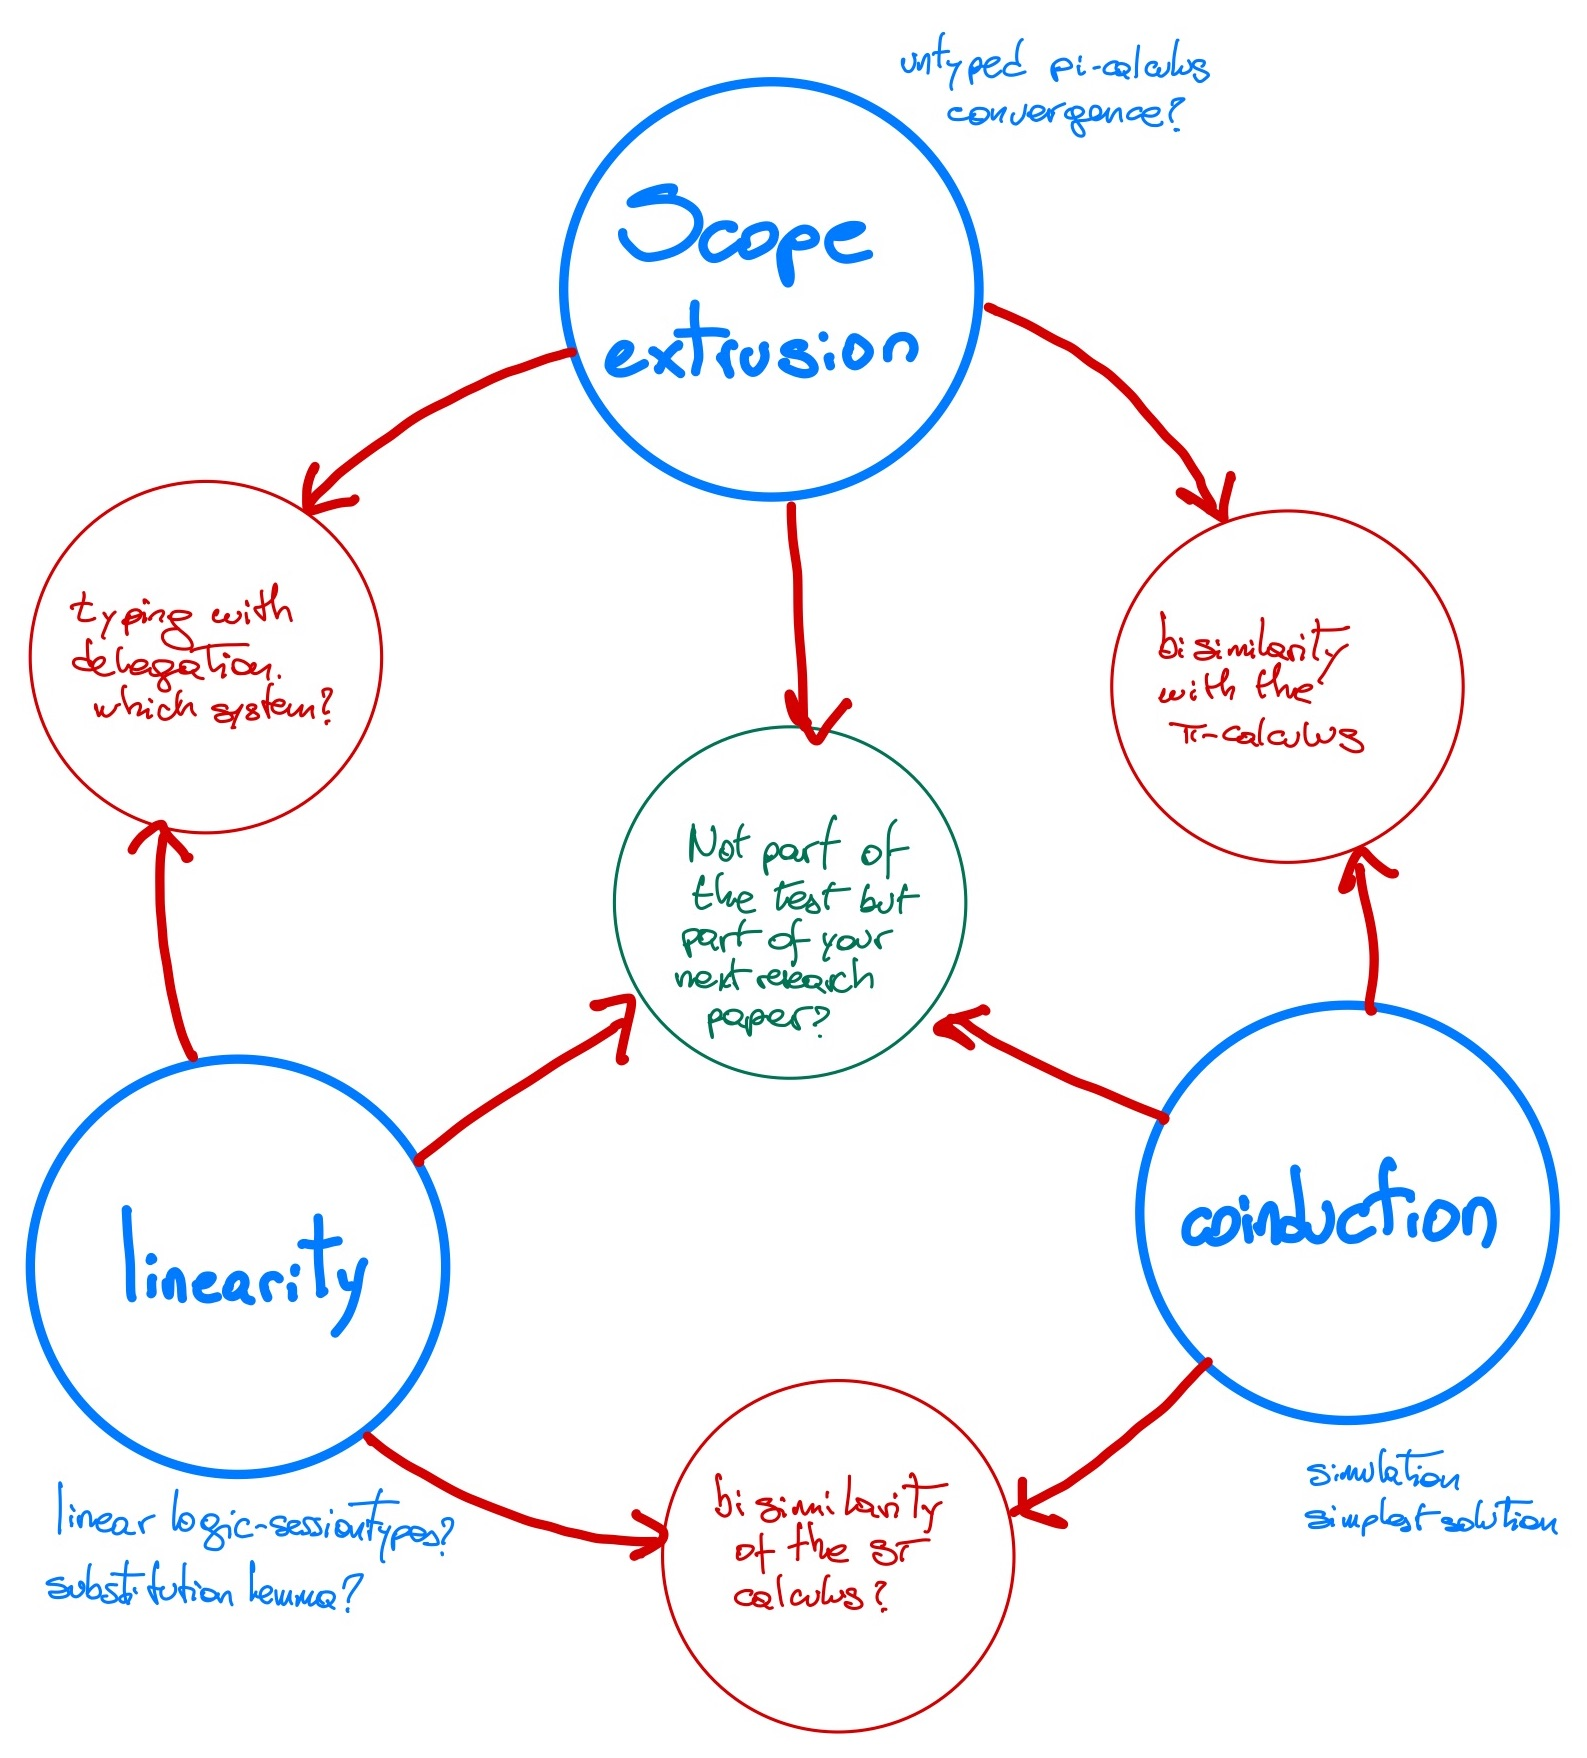
\includegraphics[width=0.75\textwidth]{images/benchmark.jpeg}
  \caption{The benchmark's big picture.}
  \label{fig:bigpic}
\end{figure}

The big picture for the benchmark can be seen in \cref{fig:bigpic}
where the three pillars (i.e.: concepts typically needed for process
calculus proofs) appear in blue, with some ideas of what to prove. And
a second step of combining the three aspects (for a total of six steps
for the whole benchmark), and of course the $+1$-step for the
combination of everything on the reader's next research papers.

\long\def\ednote#1{\footnote{[{\it #1\/}]}\message{ednote!}}
%\long\def\ednote#1{\begin{quote}[{\it #1\/}]\end{quote}\message{note!}}
\newenvironment{metanote}{\begin{quote}\message{note!}[\begingroup\it}%
                         {\endgroup]\end{quote}}
\long\def\ignore#1{}

\subsection{Preliminaries}
\label{sec:prelim}

We list here some common notions that we will use in the following. Since the calculi under study are somewhat different, we will note in each section which will apply.

We assume the existence of some type of \emph{base values}, represented by the symbols
\( a, b, \dots \), the existence of some type
of \emph{variable names}, represented by the symbols
\( l, m, \dots \), and the existence of some type of \emph{names},
represented by the symbols \( x, y, \dots \). \ednote{AM: are we assuming that names can be compared for equality everywhere or only in C2?} % 

The syntax of processes will include:
the process \( \Pend \) or \emph{inaction}, a process which can do nothing. The process \( \Ppar{P}{Q} \) is the \emph{composition} of process \( P \) and process \( Q \).
The two components can proceed independently of each other, or they can interact via shared names. The process \( \Pchoice{P}{Q} \) is a non-deterministic \emph{choice} between continuing as the process \( P \) or as the process \( Q \).

For communication, processes include \emph{input} and \emph{output}, whose
signature will depend on the calculus being value or name-passing.
We use here the metavariables $c,k$ to abstract over this choice.
The process \( \Pout{x}{c}{P} \) is an \emph{output}, which can send
\( c \) via \( x \), then continue as \( P \).  % The intention is that
% the value \( v \) must be a base value when it is actually sent, and
% this will be enforced in the semantics later on
The process \( \Pin{x}{k}{P} \) is an \emph{input}, which can receive a $c$
via \( x \), then continue as \( P \) with the received element
substituted for \( k \).  The input operator thus
binds \( k \) in \( P \).

The process \( \Pres{x}{P} \) is the \emph{restriction} of the name
\( x \) to \( P \), binding \( x \) in \( P \).


The process \( \Preplicate{P} \) is the \emph{replication} of the process \( P \).
It can be thought of as the infinite composition \( \Ppar{P}{\Ppar{P}{\cdots}} \).
Replication makes it possible to express infinite behaviors.

We will use the notation \( \freenames{P} \) to denote the set of
names that occur free,
% (i.e.\ not bound by a restriction) in \( P \),
\( \boundnames{P} \) to denote the set of names that occur bound
% (by a restriction)
in \( P \) and  \( \freevars{P} \)
to denote the set of variable names that occur free
% (i.e.\ not bound by an input)
in \( P \).  We will use the notation \( \boundvars{P} \)
for the set of variable names that occur bound
% (by an input)
in \( P \).  We will use the notation \( \subst{P}{v}{l} \) to denote
the process \( P \) with value \( v \) substituted for variable name
\( l \). Similarly, \( \subst{P}{x}{y} \) denotes the process
\( P \) with name \( x \) substituted for name \( y \).


Two processes \( P \) and \( Q \) are \( \alpha \)-convertible,
written \( \alphacon{P}{Q} \), if \( Q \) can be obtained from \( P \)
by a finite number of substitutions of bound variable names.  As a
convention, we will identify \( \alpha \)-convertible processes and we
assume that bound names and bound variable names of any processes are
chosen to be different from the names and variable names that occur
free in any other entities under consideration, such as processes,
substitutions, and sets of names or variable names.  This is justified
because any overlapping names and variable names may be
\( \alpha \)-converted such that the assumption is satisfied.


A \emph{context} is obtained by taking a process and replacing a single occurrence of \( \Pend \) in it with the special \emph{hole} symbol \( \ctxhole \).
As a convention, we do \emph{not} identify \( \alpha \)-convertible contexts.

We will think of contexts as functions between processes.
A context \( C \) can be \emph{applied} to a process \( P \), written \( \applyctx{C}{P} \), by replacing the hole in C by \( P \), thus obtaining another process.
The replacement should be literal, so names and variable names that are free in \( P \) can become bound in \( \applyctx{C}{P} \).

We say that an equivalence relation \( \mathcal{S} \) is a \emph{congruence} if \( (P,Q) \in \mathcal{S} \) implies that for any context \( C \), \( (\applyctx{C}{P}, \applyctx{C}{Q}) \in \mathcal{S} \).

\subsection{Challenge: Linearity and behavioral type systems}
\label{sec:challenge:linearity-beh-types}

This challenge formalises a proof that requires reasoning about linearity of channels.
Linearity is the notion that a channel must be used exactly once in a process.
This is necessary to prove properties about session type systems.
Linear reasoning is also necessary to formalise e.g.\ linear and affine types for the pi-calculus and cut elimination in linear logics.

The setting for this challenge is a small calculus with a session type system, the syntax and semantics of which are presented below.
The objective of this challenge is to prove type preservation (also known as subject reduction) for the type system, i.e.\ that well-typed processes can only transition to processes which are also well-typed in the same context.

\subsubsection{Syntax}

% We assume the existence of some type of \emph{base values}, values of which we will denote by \( a, b, \dots \), the existence of some type of \emph{variable names}, values of which we will denote by \( l, m, \dots \), and the existence of some type of \emph{names}, values of which we will denote by \( x, y, \dots \).
% We assume the existence of some type of \emph{base values}, represented by the symbols
%  \( a, b, \dots \), the existence of some type
% of \emph{variable names}, represented by the symbols
% \( l, m, \dots \), and the existence of some type of \emph{names},
% represented by the symbols \( x, y, \dots \).

The syntax is
given by the grammar:
\begin{metanote}
AM:  Should we save some space like this?
\end{metanote}
% \begin{align*}
%   v,w :=&&& a \\
%   |&&& l \\
%   P,Q :=&&& \Pend \\
%   |&&& \Pout{x}{v}{P} \\
%   |&&& \Pin{x}{l}{P} \\
%   |&&& \Ppar{P}{Q} \\
%   |&&& \Presd{x}{y}{P}
         %   \end{align*}
% \newcommand{\bmid}{\mathbf{\Vert}}
\[
\begin{array}{rcl}
  v,w & ::= & a \mid l \\
   P,Q & ::=& \Pend \mid \Pout{x}{v}{P} \mid \Pin{x}{l}{P} \mid \PBpar{P}{Q} \mid  \Presd{x}{y}{P}
\end{array}
\]
A \emph{value} \( v, w, \dots \) is either a base value \( a \) or a variable name \( l \).
% The process \( \Pend \) is \emph{inaction}: a process which can do nothing.
The output process \( \Pout{x}{v}{P} \) sends the value \( v \) via \( x \), then continue as \( P \).
The intention is that the value \( v \) must be a base value when it is actually sent, and this will be enforced in the semantics later on.
The input process \( \Pin{x}{l}{P} \) is an \emph{input}, which can receive a base value via \( x \), then continue as \( P \) with the received value substituted for the variable name \( l \).
% The input operator thus binds the variable name \( l \) in \( P \).
% The process \( \Ppar{P}{Q} \) is the \emph{composition} of process \( P \) and process \( Q \).
% The two components can proceed independently of each other, or they can interact via shared names.
The process \( \Presd{x}{y}{P} \) is the \emph{restriction} of the channel with endpoints named \( x \) and \( y \) to \( P \).
Components in \( P \) can use the names \( x \) and \( y \) to interact with each other (sending on \( x \) and receiving on \( y \) or vice versa), but not with processes outside of the restriction.
The restriction operator thus binds the names \( x \) and \( y \) in \( P \).
Note that the scope of a restriction may not change when processes interact, since it is only possible to send and receive values, and not names.
Note that there is no recursion of replication in the syntax, and thus no infinite behaviors can be expressed.

% We will use the notation \( \freenames{P} \) to denote the set of names that occur free (i.e.\ not bound by a restriction) in \( P \).
% We will use the notation \( \boundnames{P} \) to denote the set of names that occur bound (by a restriction) in \( P \).
% We will use the notation \( \freevars{P} \) to denote the set of variable names that occur free (i.e.\ not bound by an input) in \( P \).
% We will use the notation \( \boundvars{P} \) to denote the set of variable names that occur bound (by an input) in \( P \).
% We will use the notation \( \subst{P}{v}{l} \) to denote the process \( P \) with value \( v \) substituted for variable name \( l \).

% Two processes \( P \) and \( Q \) are \( \alpha \)-convertible, written \( \alphacon{P}{Q} \), if \( Q \) can be obtained from \( P \) by a finite number of substitutions of bound variable names.
% As a convention, we will identify \( \alpha \)-convertible processes.

% As a convention, we assume that bound names and bound variable names of any processes are chosen to be different from the names and variable names that occur free in any other entities under consideration, such as processes, substitutions, and sets of names or variable names.
% This is justified because any overlapping names and variable names may be \( \alpha \)-converted such that the assumption is satisfied.

\subsubsection{Semantics}
We describe the actions that the system can perform using a small step operational semantics.
To simplify the definition of the reduction relation, we will first factor out a structural congruence relation on processes, and for this we need a few definitions.

\subsubsection{Contexts and congruences}
% A \emph{context} is obtained by taking a process and replacing a single occurrence of \( \Pend \) in it with the special \emph{hole} symbol \( \ctxhole \).
% As a convention, we do \emph{not} identify \( \alpha \)-convertible contexts.

% We will think of contexts as functions between processes.
% A context \( C \) can be \emph{applied} to a process \( P \), written \( \applyctx{C}{P} \), by replacing the hole in C by \( P \), thus obtaining another process.
% The replacement should be literal, so names and variable names that are free in \( P \) can become bound in \( \applyctx{C}{P} \).

% We say that an equivalence relation \( \mathcal{S} \) is a \emph{congruence} if \( (P,Q) \in \mathcal{S} \) implies that for any context \( C \), \( (\applyctx{C}{P}, \applyctx{C}{Q}) \in \mathcal{S} \).

\emph{Structural congruence} is the smallest congruence relation that satisfies the following axioms:
\begin{mathpar}
  \inferrule[Sc-Par-Comm]{ }{\scong{\Ppar{P}{Q}}{\Ppar{Q}{P}}}
  \and
  \inferrule[Sc-Par-Assoc]{ }{\scong{\Ppar{(\Ppar{P}{Q})}{R}}{\Ppar{P}{(\Ppar{Q}{R})}}}
  \and
  \inferrule[Sc-Par-Inact]{ }{\scong{\Ppar{P}{\Pend}}{P}}
  \and
  \inferrule[Sc-Res-Par]{\{x,y\} \cap \freenames{Q} = \emptyset}{\scong{\Ppar{\Presd{x}{y}{P}}{Q}}{\Presd{x}{y}{(\Ppar{P}{Q})}}}
  \and
  \inferrule[Sc-Res-Inact]{ }{\scong{\Presd{x}{y}{\Pend}}{\Pend}}
  \and
  \inferrule[Sc-Res]{ }{\scong{\Presd{x_1}{y_1}{\Presd{x_2}{y_2}{P}}}{\Presd{x_2}{y_2}{\Presd{x_1}{y_1}{P}}}}
\end{mathpar}

The operational semantics is then defined as the following binary relation on processes:
\begin{mathpar}
  \inferrule[R-Com]{ }{\reduces{\Presd{x}{y}{(\Ppar{\Pout{x}{v}{P}}{\Ppar{\Pin{y}{l}{Q}}{R}})}}{\Presd{x}{y}{(\Ppar{P}{\Ppar{\subst{Q}{v}{l}}{R}})}}}
  \and
  \inferrule[R-Res]{\reduces{P}{Q}}{\reduces{\Presd{x}{y}{P}}{\Presd{x}{y}{Q}}}
  \and
  \inferrule[R-Par]{\reduces{P}{Q}}{\reduces{\Ppar{P}{R}}{\Ppar{Q}{R}}}
  \and
  \inferrule[R-Struct]{\scong{P}{P'} \\ \reduces{P'}{Q'} \\ \scong{Q}{Q'}}{\reduces{P}{Q}}
\end{mathpar}
Note that there is no rule for inferring an action of an input or output process except those that match the input/output capability.
Note also that due to rule \TirName{R-Com}, the process \( \Pin{y}{l}{P} \) can receive \emph{any} base value.
On the other hand, since the rule \TirName{R-Com} only applies to sending base values, there is no way to send a variable name or a name.

\subsubsection{Session types}
Our process syntax allows us to write processes that are not well-formed in the sense that they either use the endpoints bound by a restriction to communicate in a way that does not follow the intended duality of communication, or attempt to send something which is not a base value.
As an example, the following process attempts to send a base value on both \( x \) and \( y\), whereas the intention of restricting names is that one of the names is used for sending and the other for receiving: \( \Presd{x}{y}{(\Ppar{\Pout{x}{a}{\Pend}}{\Pout{y}{a}{\Pend}})} \).
Another example is the following process, which attempts to send a variable that is not resolved at the time of sending: \( \Presd{x}{y}{(\Ppar{\Pout{x}{l}{\Pend}}{\Pin{y}{l}{\Pend}})} \).

To alleviate this issue, we introduce a \emph{session type system}, which will detect processes that are not well-formed.
To this end, we need to first formally define what we mean by well-formed.
We say that a process \( P \) is \emph{prefixed at variable \( x \)} if it is of the form \( \Pout{x}{v}{P} \) or \( \Pin{x}{l}{P} \).
A process is then \emph{well-formed} if, for each of its structurally congruent processes of the form \( \Presd{x_1}{y_1}{\dots \Presd{x_n}{y_n}{(\Ppar{\Ppar{P}{Q}}{R})}} \), with \( n \geq 0 \), it holds that, if \( P \) is prefixed at \( x_1 \) and \( Q \) is prefixed at \( y_1 \), then \( \Ppar{P}{Q} \) is of the form \( \Ppar{\Pout{x_1}{a}{P'}}{\Pin{y_1}{l}{Q'}} \).

Note that well-formed processes do not necessarily reduce, since e.g.\ the process
\begin{equation*}
  \Presd{x_1}{y_1}{\Presd{x_2}{y_2}{(\Ppar{\Pout{x_1}{a}{\Pin{y_2}{l}{\Pend}}}{\Pout{y_2}{x_2}{\Pin{y_1}{l}{\Pend}}})}}
\end{equation*}
is well-formed, but has no reduction.
\paragraph{Syntax}
Our type system does not type processes directly, but instead focuses on the channels used in the process.
The syntax of \emph{session types} \( S, T \) and \emph{type contexts} \( \Gamma \) is as follows:
\begin{align*}
  S,T := &&& \Tend \\
  |&&& \Tbase \\
  |&&& \Tin{S} \\
  |&&& \Tout{S} \\
  \Gamma := &&& \Cempty \\
  |&&& \Cadd{\Gamma}{\hastype{x}{S}}
       %% AM: added
        \\
  |&&& \Cadd{\Gamma}{\hastype{l}{S}}
\end{align*}
The \emph{end type}, \( \Tend \), is the type of an endpoint on which no further interaction is possible.
The \emph{base type}, \( \Tbase \), is the type of base values.
The \emph{input type}, \( \Tin{S} \), is the type of an endpoint which is ready to receive a value, then continue with type \( S \).
The \emph{output type}, \( \Tout{S} \), is the type of an endpoint which is ready to send a value, then continue with type \( S \).

Typing contexts gather type information about names.
The \emph{empty type context}, \( \Cempty \), does not contain any information.
The \emph{type context with \( x \) added}, \( \Cadd{\Gamma}{\hastype{x}{T}} \) adds the information that \( x \) has type \( T \) to the existing type context \( \Gamma \).
All of the names added to a type context must be distinct.
We treat type contexts as sets, not ordered lists, and the order in which information is added to a type context thus does not matter.

Since we need to determine whether endpoints are used dually to determine whether processes are well-formed, we will need to formally define the dual of a type.
The dual of a type, \( \dual{T} \), is defined by the following equations:
\begin{mathpar}
  \inferrule{}{\dual{\Tin{S}} = \Tout{\dual{S}}}
  \and
  \inferrule{}{\dual{\Tout{S}} = \Tin{\dual{S}}}
  \and
  \inferrule{}{\dual{\Tend} = \Tend}
\end{mathpar}
Note that the dual function is not total, since it is not defined for base types.

\paragraph{Splitting and updating contexts}
Our type system will maintain two invariants:
\begin{enumerate}
\item Endpoints are used exactly once
\item Endpoints that are part of the same restriction have dual types
\end{enumerate}
The first invariant is maintained by linearly splitting type contexts when typing compositions of processes.
The second invariant is maintained by requiring duality when typing restrictions.

To keep track of linearity, we introduce two \emph{qualifiers}: \( \un{T} \) and \( \lin{T} \).
A type is \emph{unrestricted}, \( \un{T} \), if and only if \( T = \Tbase \) or \( T = \Tend \).
All types are \emph{linear}, \( \lin{T} \).
The qualifiers extend to contexts in the following way: \( q(\Gamma) \) if and only if \( \hastype{x}{T} \in \Gamma \) implies \( q(T) \).

The \emph{linear split} of a context, \( \Gamma = \Csplit{\Gamma_1}{\Gamma_2} \), is defined by the following rules:
\begin{mathpar}
  \inferrule[Split-Empty]{ }{\Cempty = \Csplit{\Cempty}{\Cempty}}
  \and
  \inferrule[Split-Un]{\Csplit{\Gamma_1}{\Gamma_2} = \Gamma \\ \un{T}}{\Cadd{\Gamma}{\hastype{x}{T}} = \Csplit{(\Cadd{\Gamma_1}{\hastype{x}{T}})}{(\Cadd{\Gamma_2}{\hastype{x}{T}})}}
  \and
  \inferrule[Split-Lin-L]{\Gamma = \Csplit{\Gamma_1}{\Gamma_2}}{\Cadd{\Gamma}{\hastype{x}{S}} = \Csplit{(\Cadd{\Gamma_1}{\hastype{x}{S}})}{\Gamma_2}}
  \and
  \inferrule[Split-Lin-R]{\Gamma = \Csplit{\Gamma_2}{\Gamma_2}}{\Cadd{\Gamma}{\hastype{x}{S}} = \Csplit{\Gamma_1}{(\Cadd{\Gamma_2}{\hastype{x}{S}})}}
\end{mathpar}

We will also need to update contexts with new type information in a safe way while typing input and output.
The \emph{context update}, \( \Cupdate{\Gamma}{\hastype{x}{T}} = \Gamma' \), is defined by the following rules:
\begin{mathpar}
  \inferrule[Update-Name]{\hastype{x}{U} \notin \Gamma}{\Cupdate{\Gamma}{\hastype{x}{T}} = \Cadd{\Gamma}{\hastype{x}{T}}}
  \and
  \inferrule[Update-Un]{\un{T}}{\Cupdate{(\Cadd{\Gamma}{\hastype{x}{T}})}{\hastype{x}{T}} = (\Cadd{\Gamma}{\hastype{x}{T}})}
\end{mathpar}

\subsubsection{Typing rules}
We have three typing judgments: one for values, one for names, and one for processes.
The typing rules for values are as follows:
\begin{mathpar}
  \inferrule[T-Base]{\un{\Gamma}}{\types{\Gamma}{\hastype{a}{\Tbase}}}
  \and
  \inferrule[T-Var]{\un{\Gamma}}{\types{\Cadd{\Gamma}{\hastype{l}{\Tbase}}}{\hastype{l}{\Tbase}}}
\end{mathpar}
The only typing rule for names is:
\begin{mathpar}
  \inferrule[T-Name]{\un{\Gamma}}{\types{\Cadd{\Gamma}{\hastype{x}{T}}}{\hastype{x}{T}}}
\end{mathpar}
The typing rules for processes are as follows:
\begin{mathpar}
  \inferrule[T-Inact]{\un{\Gamma}}{\types{\Gamma}{\Pend}}
  \and
  \inferrule[T-Par]{\types{\Gamma_1}{P} \\ \types{\Gamma_2}{Q}}{\types{\Csplit{\Gamma_1}{\Gamma_2}}{\Ppar{P}{Q}}}
  \and
  \inferrule[T-Res]{\types{\Cadd{\Cadd{\Gamma}{\hastype{x}{T}}}{\hastype{y}{\dual{T}}}}{P}}{\types{\Gamma}{\Presd{x}{y}{P}}}
  \and
  \inferrule[T-Out]{\types{\Gamma_1}{\hastype{x}{\Tout{T}}} \\ \types{\Gamma_2}{\hastype{v}{\Tbase}} \\ \types{\Cupdate{\Gamma_3}{\hastype{x}{T}}}{P}}{\types{\Csplit{\Gamma_1}{\Csplit{\Gamma_2}{\Gamma_3}}}{\Pout{x}{v}{P}}}
  \and
  \inferrule[T-In]{\types{\Gamma_1}{\hastype{x}{\Tin{U}}} \\ \types{\Cupdate{(\Cadd{\Gamma_2}{\hastype{l}{\Tbase}})}{\hastype{x}{U}}}{P}}{\types{\Csplit{\Gamma_1}{\Gamma_2}}{\Pin{x}{l}{P}}}
\end{mathpar}

\subsubsection{Challenge}
The objective of this challenge is to prove the following theorems:
\begin{theorem}
  If \( \types{\Gamma}{P} \) and \( \reduces{P}{Q} \) then \( \types{\Gamma}{Q} \).
\end{theorem}

\begin{theorem}
  If \( \types{\Cempty}{P} \), then \( P \) is well-formed.
\end{theorem}

\begin{corollary}
  If \( \types{\Cempty}{P} \) and \( \reduces{P}{Q} \) then \( Q \) is well-formed.
\end{corollary}

The following lemmas may be of use:
\begin{lemma}
  If \( \types{\Gamma}{P} \) and \( \un{T} \) then \( \types{\Cadd{\Gamma}{\hastype{x}{T}}}{P} \).
\end{lemma}

\begin{lemma}
  Assume \( \types{\Gamma}{P} \) and \( x \notin \freenames{P} \).
  Then:
  \begin{enumerate}
  \item \( \hastype{x}{\Tout{T}} \notin \Gamma \).
  \item \( \hastype{x}{\Tin{T}} \notin \Gamma \).
  \item if \( \Gamma = \Cadd{\Gamma'}{\hastype{x}{T}} \) then \( \types{\Gamma'}{P} \).
  \end{enumerate}
\end{lemma}

\begin{lemma}
  If \( \types{\Gamma}{P} \) and \( \scong{P}{Q} \) then \( \types{\Gamma}{Q} \).
\end{lemma}

\begin{lemma}
  If \( \types{\Gamma_1}{\hastype{v}{T}} \) and \( \types{\Cadd{\Gamma_2}{\hastype{x}{T}}}{P} \) and \( \Gamma = \Csplit{\Gamma_1}{\Gamma_2} \) then \( \types{\Gamma}{\subst{v}{x}{P}} \).
\end{lemma}

\subsection{Challenge: Name passing and scope extrusion}
\label{sec:challenge:name-passing-scope-extrusion}

This challenge formalises a proof that requires explicit scope extrusion.
Scope extrusion is the notion that a process can send restricted names to another process, as long as the restriction can safely be ``extruded'' (i.e.\ expanded) to include the receiving process.
This e.g.\ allows a process to set up a private connection by sending a restricted name to another process, then using this name for further communication.

Reasoning about scope extrusion explicitly can sometimes be avoided by introducing a structural congruence rule into the semantics, but doing this means we lose information about the scope when reasoning about the semantics.
Explicitly reasoning about scope extrusion is necessary to describe e.g.\ monitors and compositions.

The setting for this challenge is an untyped \( \pi \)-calculus, the syntax and semantics of which are presented below.
We will define two different semantics for our system: one that avoids explicit reasoning about scope extrusion, and one that does not.
The objective of this challenge is to prove that the two semantics are equivalent up to structural congruence.

\subsubsection{Syntax}
In this section we assume that \emph{names}  can be compared for equality.
The syntax in this challenge will be split into two levels: processes and summations.
The syntax of processes is given by:
\begin{align*}
  P,Q :=&&& \Ppar{P}{Q} \\
  |&&& \Pres{x}{P} \\
  |&&& M
\end{align*}
The syntax of summations is given by:
\begin{align*}
  M,N :=&&& \Pend \\
  |&&& \Pout{x}{y}{P} \\
  |&&& \Pin{x}{y}{P} \\
  |&&& \Pchoice{M}{N}
\end{align*}
Splitting the syntax into these two layers has the effect of disallowing choices directly between parallel processes.
Allowing choices between arbitrary processes complicates the theory and is rarely useful.

%The process \( \Pend \) is \emph{inaction}: a process which can do nothing.
The process \( \Pout{x}{y}{P} \) is an \emph{output}, which can send the name \( y \) via \( x \), then continue as \( P \).
The process \( \Pin{x}{y}{P} \) is an \emph{input}, which can receive a name via \( x \), then continue as \( P \) with the received name substituted for \( y \).
%The input operator thus binds the name \( y \) in \( P \).
% The process \( \Ppar{P}{Q} \) is the \emph{composition} of process \( P \) and process \( Q \).
% The two components can proceed independently of each other, or they can interact via shared names.
% The process \( \Pres{x}{P} \) is the \emph{restriction} of the name \( x \) to \( P \).
% Components in \( P \) can use the name \( x \) to interact with each other, but not with processes outside of the restriction.
% The restriction operator thus binds the name \( x \) in \( P \).
Note that the scope of a restriction may change when processes interact. Namely, a restricted name may be sent \emph{outside} of its scope.
% The process \( \Pchoice{P}{Q} \) is a non-deterministic \emph{choice} between continuing as the process \( P \) or as the process \( Q \).
Note that there is no recursion or replication in the syntax, and thus no infinite behaviors can be expressed.

% We will use the notation \( \freenames{P} \) to denote the set of names that occur free (i.e.\ not bound by a restriction or an input) in \( P \).
% We will use the notation \( \boundnames{P} \) to denote the set of names that occur bound (by a restriction or an input) in \( P \).
% We will use the notation \( \subst{P}{x}{y} \) to denote the process \( P \) with \( x \) substituted for \( y \).

% Two processes \( P \) and \( Q \) are \( \alpha \)-convertible, written \( \alphacon{P}{Q} \), if \( Q \) can be obtained from \( P \) by a finite number of substitutions of bound names.
% As a convention, we will identify \( \alpha \)-convertible processes.

% As a convention, we assume that the bound names occurring in any collection of processes are chosen to be different from the free names occurring in those processes and from the names occurring in any substitutions applied to the processes.
% This is justified because any overlapping names may be \( \alpha \)-converted such that the assumption is satisfied.

Due to the syntactic levels, we will need to modify the definition of a context slightly by requiring that the \emph{hole} symbol \( \ctxhole \) does not appear directly as the left or right term in a choice.
For instance, we disallow the context \( \Pchoice{\ctxhole}{\Pin{x}{y}{\Pend}} \), but allow the context \( \Pchoice{\Pout{x}{z}{\ctxhole}}{\Pin{x}{y}{\Pend}} \).

\subsubsection{Reduction semantics}
The first semantics is an operational reduction semantics, which avoids reasoning explicitly about scope extrusion by way of a structural congruence rule.
\emph{Structural congruence} is the smallest congruence relation that satisfies the following axioms:
\begin{mathpar}
  \inferrule[Sc-Sum-Assoc]{ }{\scong{\Pchoice{M}{(\Pchoice{N}{L})}}{\Pchoice{(\Pchoice{M}{N})}{L}}}
  \and
  \inferrule[Sc-Sum-Comm]{ }{\scong{\Pchoice{M}{N}}{\Pchoice{N}{M}}}
  \and
  \inferrule[Sc-Sum-Inact]{ }{\scong{\Pchoice{M}{\Pend}}{M}}
  \and
  \inferrule[Sc-Par-Assoc]{ }{\scong{\Ppar{P}{(\Ppar{Q}{R})}}{\Ppar{(\Ppar{P}{Q})}{R}}}
  \and
  \inferrule[Sc-Par-Comm]{ }{\scong{\Ppar{P}{Q}}{\Ppar{Q}{P}}}
  \and
  \inferrule[Sc-Par-Inact]{ }{\scong{\Ppar{P}{\Pend}}{P}}
  \and
  \inferrule[Sc-Res-Par]{x \notin \freenames{Q}}{\scong{\Ppar{\Pres{x}{P}}{Q}}{\Pres{x}{(\Ppar{P}{Q})}}}
  \and
  \inferrule[Sc-Res-Inact]{ }{\scong{\Pres{x}{\Pend}}{\Pend}}
  \and
  \inferrule[Sc-Res]{ }{\scong{\Pres{x}{\Pres{y}{P}}}{\Pres{y}{\Pres{x}{P}}}}
\end{mathpar}

The operational semantics is then defined as the following binary relation on processes:
\begin{mathpar}
  \inferrule[R-Com]{ }{\reduces{\Ppar{(\Pchoice{\Pout{x}{y}{P}}{M})}{(\Pchoice{\Pin{x}{z}{Q}}{N})}}{\Ppar{P}{\subst{Q}{y}{z}}}}
  \and
  \inferrule[R-Res]{\reduces{P}{Q}}{\reduces{\Pres{x}{P}}{\Pres{x}{Q}}}
  \and
  \inferrule[R-Par]{\reduces{P}{Q}}{\reduces{\Ppar{P}{R}}{\Ppar{Q}{R}}}
  \and
  \inferrule[R-Struct]{\scong{P}{P'} \\ \reduces{P'}{Q'} \\ \scong{Q}{Q'}}{\reduces{P}{Q}}
\end{mathpar}
Note that there is no rule for inferring an action of an input or output process except those that match the input/output capability.
Note also that due to rule \TirName{R-Com}, the process \( \Pin{x}{z}{P} \) can receive \emph{any} name.
Finally, note that rule \TirName{R-Struct} allows for applying the structural congruence both before and after the reduction.
This ensures that the reduction relation is closed under structural congruence.

\subsubsection{Transition system semantics}
The second semantics of the system describe the actions that the system can perform by defining a labelled transition relation on processes.
The transitions are labelled by \emph{actions}, the syntax of which is as follows:
\begin{align*}
  \alpha := &&& \Aoutf{x}{y} \\
  |&&& \Ain{x}{y} \\
  |&&& \Aoutb{x}{y} \\
  |&&& \Atau
\end{align*}
The \emph{free output action} \( \Aoutf{x}{y} \) is sending the name \( y \) via \( x \).
The \emph{input action} \( \Ain{x}{y} \) is receiving the name \( y \) via \( x \).
The \emph{bound output action} \( \Aoutb{x}{y} \) is sending a fresh name \( y \) via \( x \).
The \emph{internal action} \( \Atau \) is performing some unobservable action, e.g.\ internal communication.

We will extend the notion of free and bound occurrences with 
\( \freenames{\alpha} \) to denote the set of names that occur free in
the action \( \alpha \) and  \( \boundnames{\alpha} \) to
denote the set of names that occur bound in the action \( \alpha \).
In the free output action \( \Aoutf{x}{y} \) and the input action
\( \Ain{x}{y} \), both \( x \) and \( y \) are free names.  In the
bound output action \( \Aoutb{x}{y} \), \( x \) is a free name, while
\( y \) is a bound name.  We will further use the notation
\( \names{\alpha} \) to denote the union of \( \freenames{\alpha} \)
and \( \boundnames{\alpha} \), i.e.\ the set of all names that occur
in the action \( \alpha \).

The transition relation is then defined by the following rules:
\begin{mathpar}
  \inferrule[Out]{ }{\transition{\Pout{x}{y}{P}}{\Aoutf{x}{y}}{P}}
  \and
  \inferrule[In]{ }{\transition{\Pin{x}{z}{P}}{\Ain{x}{y}}{\subst{P}{y}{z}}}
  \and
  \inferrule[Sum-L]{\transition{P}{\alpha}{P'}}{\transition{\Pchoice{P}{Q}}{\alpha}{P'}}
  \and
  \inferrule[Sum-R]{\transition{P}{\alpha}{P'}}{\transition{\Pchoice{Q}{P}}{\alpha}{P'}}
  \and
  \inferrule[Par-L]{\transition{P}{\alpha}{P'} \\ \boundnames{\alpha} \cap \freenames{Q} = \emptyset}{\transition{\Ppar{P}{Q}}{\alpha}{\Ppar{P'}{Q}}}
  \and
  \inferrule[Par-R]{\transition{Q}{\alpha}{Q'} \\ \boundnames{\alpha} \cap \freenames{P} = \emptyset}{\transition{\Ppar{P}{Q}}{\alpha}{\Ppar{P}{Q'}}}
  \and
  \inferrule[Comm-L]{\transition{P}{\Aoutf{x}{y}}{P'} \\ \transition{Q}{\Ain{x}{y}}{Q'}}{\transition{\Ppar{P}{Q}}{\Atau}{\Ppar{P'}{Q'}}}
  \and
  \inferrule[Comm-R]{\transition{P}{\Ain{x}{y}}{P'} \\ \transition{Q}{\Aoutf{x}{y}}{Q'}}{\transition{\Ppar{P}{Q}}{\Atau}{\Ppar{P'}{Q'}}}
  \and
  \inferrule[Close-L]{\transition{P}{\Aoutb{x}{z}}{P'} \\ \transition{Q}{\Ain{x}{z}}{Q'} \\ z \notin \freenames{Q}}{\transition{\Ppar{P}{Q}}{\tau}{\Pres{z}{\Ppar{P'}{Q'}}}}
  \and
  \inferrule[Open]{\transition{P}{\Aoutf{x}{z}}{P'} \\ z \neq x}{\transition{\Pres{z}{P}}{\Aoutb{x}{z}}{P'}}
  \and
  \inferrule[Close-R]{\transition{P}{\Ain{x}{z}}{P'} \\ \transition{Q}{\Aoutb{x}{z}}{Q'} \\ z \notin \freenames{P}}{\transition{\Ppar{P}{Q}}{\tau}{\Pres{z}{\Ppar{P'}{Q'}}}}
  \and
  \inferrule[Res]{\transition{P}{\alpha}{P'} \\ z \notin \names{\alpha}}{\transition{\Pres{z}{P}}{\alpha}{\Pres{z}{P'}}}
\end{mathpar}
Note that there is no rule for inferring transitions from \( \Pend \), and that there is no rule for inferring an action of an input or output process except those that match the input/output capability.
Note also that due to rule \TirName{In}, the process \( \Pin{x}{z}{P} \) can receive \emph{any} name.

We keep the convention that bound names of any processes or actions
are chosen to be different from the names that occur free in any other
entities under consideration, such as processes, actions,
substitutions, and sets of names.  The convention has one exception,
namely that in the transition \( \transition{P}{\Aoutb{x}{z}}{Q} \),
the name \( z \) (which occurs bound in \( P \) and the action
\( \Aoutb{x}{z} \)) may occur free in \( Q \).  Without this exception
it would be impossible to express scope extrusion.

\subsubsection{Challenge}
\begin{lemma}\label{se-lemma-harmony-fact}
  If \( \scong{P}{Q} \) and \( \transition{P}{\alpha}{P'} \), then for some \( Q' \) we have \( \transition{Q}{\alpha}{Q'} \) and \( \scong{P'}{Q'} \).
\end{lemma}
\begin{proof}
  Sketch. First, show the special case when \( P \) can be rewritten to \( Q \) with a single application of an axiom of the structural congruence to some subterm of P.
  The proof is then by induction on the number of such steps.
\end{proof}

\begin{lemma}\label{se-lemma-normalized-reduction}
  If \( \reduces{P}{Q} \) then there are \( x, y, z, z_1, \dots, z_n, R_1, N_1, R_2, N_2, \) and \( S\) such that
  \begin{align*}
    &\scong{P}{\Pres{z_1}{\!\dots \Pres{z_n}{(\Ppar{(\Ppar{(\Pchoice{\Pout{x}{y}{R_1}}{N_1})}{(\Pchoice{\Pin{x}{z}{R_2}}{N_2})})}{S})}}} \\
    &\scong{Q}{\Pres{z_1}{\!\dots \Pres{z_n}{(\Ppar{(\Ppar{R_1}{\subst{R_2}{y}{z}})}{S})}}}
  \end{align*}
\end{lemma}
To prove this lemma, we introduce the notion of a \emph{normalized derivation} of a reduction \( \reduces{P}{Q} \), which is of the following form.
The first rule applied is \TirName{R-Com}. The derivation continues with an application of \TirName{R-Par}, followed by zero or more applications of \TirName{R-Res}.
The last rule is an application of \TirName{R-Struct}.
\begin{lemma}\label{se-lemma-normalized-derivation}
  Every reduction has a normalized derivation.
\end{lemma}
\begin{proof}
  Sketch. To obtain a normalized derivation from an arbitrary derivation we will need to check that rules \TirName{R-Com}, \TirName{R-Par} and \TirName{R-Res} commute with \TirName{R-Struct}, and that two applications of \TirName{R-Struct} can be combined into one.
\end{proof}
\begin{proof}{Of lemma \autoref{se-lemma-normalized-reduction}.}
  Follows immediately from lemma \autoref{se-lemma-normalized-derivation} and the shape of a normalized derivation.
\end{proof}

The objective of this challenge is to prove the following theorems, which together show the equivalence between the reduction semantics and the transition system semantics up to structural congruence.
The first of the theorems involves reasoning about scope extrusion more directly than the other, and if time does not permit proving both of the theorems, \autoref{thm:se-trans-implies-red} should be proven first.
\begin{theorem}\label{thm:se-trans-implies-red}
  \( \transition{P}{\Atau}{Q} \) implies \( \reduces{P}{Q} \).
\end{theorem}
\begin{proof}
  The proof is by induction on the inference of \( \transition{P}{\Atau}{Q} \) using the following:
  \begin{enumerate}
  \item if \( \transition{Q}{\Aoutf{x}{y}}{Q'} \) then \( \scong{Q}{\Pres{w_1}{\!\dots \Pres{w_n}{(\Ppar{(\Pchoice{\Pout{x}{y}{R}}{M})}{S})}}} \) and \( \scong{Q'}{\Pres{w_1}{\!\dots \Pres{w_n}{(\Ppar{R}{S})}}} \) where \( x,y \notin \{ w_1, \dots, w_n \} \).
  \item if \( \transition{Q}{\Aoutb{x}{z}}{Q'} \) then \( \scong{Q}{\Pres{z}{\Pres{w_1}{\!\dots \Pres{w_n}{(\Ppar{(\Pchoice{\Pout{x}{z}{R}}{M})}{S})}}}} \) and \( \scong{Q'}{\Pres{w_1}{\!\dots \Pres{w_n}{(\Ppar{R}{S})}}} \) where \( x \notin \{ z, w_1, \dots, w_n \} \).
  \item if \( \transition{Q}{\Ain{x}{y}}{Q'} \) then \( \scong{Q}{\Pres{w_1}{\!\dots \Pres{w_n}{(\Ppar{(\Pchoice{\Pin{x}{z}{R}}{M})}{S})}}} \) and \( \scong{Q'}{\Pres{w_1}{\!\dots \Pres{w_n}{(\Ppar{\subst{R}{y}{z}}{S})}}} \) where \( x \notin \{ w_1, \dots, w_n \} \).
  \end{enumerate}
\end{proof}

\begin{theorem}
  \( \reduces{P}{Q} \) implies the existence of a \( Q' \) such that \( \transition{P}{\Atau}{Q'} \) and \( \scong{Q}{Q'} \).
\end{theorem}
\begin{proof}
  If \( \reduces{P}{Q} \), then by lemma \autoref{se-lemma-normalized-reduction}, \( \scong{P}{P'} \) with
  \begin{equation*}
    P' = \Pres{z_1}{\!\dots \Pres{z_n}{(\Ppar{(\Ppar{(\Pchoice{\Pout{x}{y}{R_1}}{N_1})}{(\Pchoice{\Pin{x}{z}{R_2}}{N_2})})}{S})}}
  \end{equation*}
  and \( \scong{Q}{Q'} \) with
  \begin{equation*}
    Q' = \Pres{z_1}{\!\dots \Pres{z_n}{(\Ppar{(\Ppar{R_1}{\subst{R_2}{y}{z}})}{S})}} \ .
  \end{equation*}
  We can easily check that \( \transition{P'}{\tau}{Q'} \) and so by lemma \autoref{se-lemma-harmony-fact}, \( \transition{P}{\tau}{Q'} \).
\end{proof}

\subsection{Challenge: Coinduction and reasoning about infinite processes}
\label{sec:challenge:coinduction}

This challenge formalises a proof that requires coinductive techniques.
Coinduction is a proof technique for infinite structures, which arise in this context due to systems with behaviors that continue indefinitely.
Coinduction is the dual of induction: whereas induction is useful for proving properties of least fixed points, coinduction is useful for proving properties of greatest fixed points.

The setting for this challenge is an untyped calculus of communicating systems with replication of processes, the syntax and semantics of which are presented below.
The objective of this challenge is to prove that strong barbed bisimulation for this calculus is an equivalence relation. Which, to reiterate, entails the use of coinduction due to the presence of infinite behavior.

\subsubsection{Syntax}
% We assume the existence of some type of \emph{base values}, values of which we will denote by \( a, b, \dots \), the existence of some type of \emph{variable names}, values of which we will denote by \( l, m, \dots \), and the existence of some type of \emph{names}, values of which we will denote by \( x, y, \dots \).
The syntax differs from \ref{sec:challenge:linearity-beh-types} for including replication and having unary restriction:
\begin{align*}
  v,w :=&&& a \\
  |&&& l \\
  P,Q :=&&& \Pend \\
  |&&& \Pout{x}{v}{P} \\
  |&&& \Pin{x}{l}{P} \\
  |&&& \Ppar{P}{Q} \\
  |&&& \Pres{x}{P} \\
  |&&& \Preplicate{P}
\end{align*}
% A \emph{value} \( v, w, \dots \) is either a base value \( a \) or a variable name \( l \).
% The process \( \Pend \) is \emph{inaction}: a process which can do nothing.
% The process \( \Pout{x}{a}{P} \) is an \emph{output}, which can send the value \( v \) via \( x \), then continue as \( P \).
% The intention is that the value \( v \) must be a base value when it is actually sent, and this will be enforced in the semantics later on.
% The process \( \Pin{x}{l}{P} \) is an \emph{input}, which can receive a base value via \( x \), then continue as \( P \) with the received value substituted for the variable name \( l \).
% The input operator thus binds the variable name \( l \) in \( P \).
% The process \( \Ppar{P}{Q} \) is the \emph{composition} of process \( P \) and process \( Q \).
% The two components can proceed independently of each other, or they can interact via shared names.
% The process \( \Pres{x}{P} \) is the \emph{restriction} of the name \( x \) to \( P \).
% Components in \( P \) can use the name \( x \) to interact with each other, but not with processes outside of the restriction.
% The restriction operator thus binds the name \( x \) in \( P \).
% Note that the scope of a restriction may not change when processes interact, since it is only possible to send and receive values, and not names.
% The process \( \Preplicate{P} \) is the \emph{replication} of the process \( P \).
% It can be thought of as the infinite composition \( \Ppar{P}{\Ppar{P}{\cdots}} \).
% Replication makes it possible to express infinite behaviours.

% We will use the notation \( \subst{P}{v}{l} \) to denote the process \( P \) with value \( v \) substituted for variable name \( l \).

% % We will use the notation \( \subst{P}{v}{w} \) to denote the process \( P \) with value \( v \) substituted for value \( w \).
% Two processes \( P \) and \( Q \) are \( \alpha \)-convertible, written \( \alphacon{P}{Q} \), if \( Q \) can be obtained from \( P \) by a finite number of substitutions of bound variable names.
% As a convention, we will identify \( \alpha \)-convertible processes.

% Also as a convention, we assume that the bound names and bound variable names occurring in any collection of processes are chosen to be different from the free names and free variable names occurring in those processes and from the names and variable names occurring in any substitutions applied to the processes.
% This is justified because any overlapping names and variable names may be \( \alpha \)-converted such that the assumption is satisfied.

\subsubsection{Semantics}
The semantics of the system describe the actions that the system can perform by defining a labelled transition relation on processes.
The transitions are labelled by \emph{actions}, the syntax of which are as follows:
\begin{align*}
  \alpha := &&& \Aoutf{x}{a} \\
  |&&& \Ain{x}{a} \\
  |&&& \Atau
\end{align*}
The \emph{output action} \( \Aoutf{x}{y} \) is sending the base value \( a \) via \( x \).
The \emph{input action} \( \Ain{x}{y} \) is receiving the base value \( y \) via \( x \).
The \emph{internal action} \( \Atau \) is performing some unobservable action, e.g.\ internal communication.

We will use the notation \( \names{\alpha} \) to denote the set of names that occur in the action \( \alpha \).

The transition relation is then defined by the following rules:
\begin{mathpar}
  \inferrule[Out]{ }{\transition{\Pout{x}{a}{P}}{\Aoutf{x}{a}}{P}}
  \and
  \inferrule[In]{ }{\transition{\Pin{x}{l}{P}}{\Ain{x}{a}}{\subst{P}{a}{l}}}
  \and
  \inferrule[Par-L]{\transition{P}{\alpha}{P'}}{\transition{\Ppar{P}{Q}}{\alpha}{\Ppar{P'}{Q}}}
  \and
  \inferrule[Par-R]{\transition{Q}{\alpha}{Q'}}{\transition{\Ppar{P}{Q}}{\alpha}{\Ppar{P}{Q'}}}
  \and
  \inferrule[Comm-L]{\transition{P}{\Aoutf{x}{a}}{P'} \\ \transition{Q}{\Ain{x}{a}}{Q'}}{\transition{\Ppar{P}{Q}}{\Atau}{\Ppar{P'}{Q'}}}
  \and
  \inferrule[Comm-R]{\transition{P}{\Ain{x}{a}}{P'} \\ \transition{Q}{\Aoutf{x}{a}}{Q'}}{\transition{\Ppar{P}{Q}}{\Atau}{\Ppar{P'}{Q'}}}
  \and
  \inferrule[Res]{\transition{P}{\alpha}{P'} \\ x \notin \names{\alpha}}{\transition{\Pres{x}{P}}{\alpha}{\Pres{x}{P'}}}
  \and
  \inferrule[Rep]{\transition{P}{\alpha}{P'}}{\transition{\Preplicate{P}}{\alpha}{\Ppar{P'}{\Preplicate{P}}}}
\end{mathpar}
Note that there is no rule for inferring transitions from \( \Pend \), and that there is no rule for inferring an action of an input or output process except those that match the input/output capability.
Note also that due to rule \TirName{In}, the process \( \Pin{x}{l}{P} \) can receive \emph{any} base value.
On the other hand, since the rule \TirName{Out} only applies to base values, there is no way to send a variable name.

% As a convention, we assume that bound names and bound variable names of any processes or actions are chosen to be different from the names and variable names that occur free in any other entities under consideration, such as processes, actions, substitutions, and sets of names or variable names.

\subsubsection{Bisimilarity}
Our notion of process equivalence relations builds on a notion of \emph{observables}.
If we allow ourselves only to observe internal transitions, we will relate either too few processes (in the strong case where we relate only processes with exactly the same number of internal transitions) or every process (in the weak case where we relate processes with any amount of internal transitions).
We must therefore allow ourselves to observe more, and here choose to define the observables of a process as the names it can use for sending and receiving.

To this end, we define the \emph{observability predicate} \( \observable{P}{\mu} \) by the following rules:
\begin{align}
  \observable{P}{\obsin{x}}  &\quad \textrm{if \( P \) can perform an input action via \( x \).} \\
  \observable{P}{\obsout{x}} &\quad \textrm{if \( P \) can perform an output action via \( x \).}
\end{align}

\emph{Strong barbed bisimilarity}, written \( \sbbisim{}{} \), is then the largest symmetric relation such that, whenever \( \sbbisim{P}{Q} \):
\begin{gather}
  \observable{P}{\mu}~\textrm{implies}~\observable{Q}{\mu} \\
  \transition{P}{\Atau}{P'}~\textrm{implies}~\transition{Q}{\Atau}{\sbbisim{}{} P'}
\end{gather}
We say that a relation is a \emph{strong barbed bisimulation} if it satisfies the conditions given above, but is not necessarily the largest such relation, and that \( P \) and \( Q \) are \emph{strong barbed bisimilar} if \( \sbbisim{P}{Q} \).
Note that, since our systems have potentially infinite behaviors, and strong barbed bisimilarity is defined as the largest relation that satisfies the conditions, bisimulation cannot be defined inductively.

\begin{theorem}
  \( \sbbisim{}{} \) is an equivalence relation, that is, the relation is reflexive, symmetric, and transitive.
\end{theorem}

Unfortunately, strong barbed bisimilarity is not a good notion of process equivalence, since it does not consider the environment of processes.
For instance, \( \sbbisim{\Pout{x}{a}{\Pout{y}{b}{\Pend}}}{\Pout{x}{a}{\Pend}} \) since \( \obsout{x} \) is the only observable in both processes and they cannot perform a \( \Atau \)-action, but \( \nsbbisim{\Ppar{\Pout{x}{a}{\Pout{y}{b}{\Pend}}}{\Pin{x}{l}{\Pend}}}{\Pout{x}{a}{\Pend}} \) since the left process can perform a \( \Atau \)-action such that \( \obsout{y} \) becomes observable, whereas the right process cannot.

% \subsubsection{Contexts and congruences}
% Before we can fix the issue with strong barbed bisimilarity, we need few more definitions.

% A \emph{context} is obtained by taking a process and replacing a single occurrence of \( \Pend \) in it with the special \emph{hole} symbol \( \ctxhole \).
% As a convention, we do \emph{not} identify \( \alpha \)-convertible contexts.

% We can think of contexts as functions between processes.
% A context \( C \) can be \emph{applied} to a process \( P \), written \( \applyctx{C}{P} \), by replacing the hole in C by \( P \), thus obtaining another process.
% The replacement should be literal, so names and variable names that are free in \( P \) can become bound in \( \applyctx{C}{P} \).

% We say that an equivalence relation \( \mathcal{S} \) is a \emph{congruence} if \( (P,Q) \in \mathcal{S} \) implies that for any context \( C \), \( (\applyctx{C}{P}, \applyctx{C}{Q}) \in \mathcal{S} \).

\subsubsection{Strong barbed congruence}
A congruence is exactly what we need to make strong barbed bisimilarity consider the environment (i.e.\ the context) of processes.

We define \emph{strong barbed congruence}, written \( \sbcong{}{} \), by saying that two processes \( P \) and \( Q \) are \emph{strong barbed congruent}, written \( \sbcong{P}{Q} \), if \( \sbbisim{\applyctx{C}{P}}{\applyctx{C}{Q}} \) for every context \( C \).

\begin{lemma}
  \( \sbcong{}{} \) is the largest congruence included in \( \sbbisim{}{} \).
\end{lemma}

\subsubsection{Challenge}
The objective of this challenge is to prove the following theorem:
\begin{theorem}
  \( \sbcong{P}{Q} \) if and only if for any process \( R \) and substitution \( \sigma \), \( \sbbisim{\Ppar{\applysubst{\sigma}{P}}{R}}{\Ppar{\applysubst{\sigma}{Q}}{R}} \).
\end{theorem}

%\paragraph{Notes about this challenge}
%Strong barbed bisimilarity is interesting by itself for this challenge, but the proof that it is an equivalence relation does not require up-to techniques, which are wide spread and interesting.
%The definition of strong barbed congruence requires introducing contexts, but this is actually nice, since they are so prevalent in the field and we want to cover as many basics as possible.
%The theorem about the strong barbed congruence requires up-to techniques, but also seems to involve introducing a structural equivalence, which is possibly not desirable.
%On the other hand, it is a nice application of structural congruence which does not ``ruin'' the semantics.



%% Local Variables:
%% mode: latex
%% TeX-master: "main"
%% End:


\section{The solutions}\label{sec:solutions}

\subsection{A tutorial solution on paper}\label{sec:tutorial}

Probably the skeleton here and more details on an appendix.

\subsection{Flexibility in solving a challenge}

\dots

\section{Future work}
\begin{itemize}
\item Multiparty session types
\item Choreography
\item Encodings
\item Code extraction
\item Conversation types
\item Psi-calculus
\item Model checking for system properties
\item More general types than session types
\end{itemize}

\section{Conclusion and related work} \label{sec:conclusion}

\bibliographystyle{plainnat}
\bibliography{references}

\label{lastpage01}

\end{document}
